\chapter{Grundlagen zu Digital Twins}

In folgendem Kapitel wird betrachtet, wie ein \ac{DT} definiert ist und welche Eigenschaften daraus ableitbar sind. Zudem wird versucht eine Unterscheidung und Abgrenzung zu einem Cyberphysischen-System vorzunehmen. Des weiteren werden verschiedene Anwendungsbereich innerhalb der Wirtschaft erläutert, welche alle von einem Einsatz digitaler Zwillinge profitieren würden. Dafür werden einige Beispiele angeführt.

\section{Was sind digitale Zwillinge?}

Innerhalb der Literatur finden sich viele verschiedene Ansätze digitale Zwillinge zu beschreiben. Dabei sticht vorallem heraus, dass oftmals nur bestimmte Teilbereiche sehr detailliert betrachten werden. Innerhalb einer Analyse von \citeauthor{barricelli2019survey} wird versucht all diese Definitionen zusammenzuführen, mit dem Ziel eine genauere Defintion eines \ac{DT}'s zu erhalten. Dafür werden insgesamt 75 Arbeiten verschiedenster Verläge ausgewertet.\autocite[S. 4, Kapitel 4]{barricelli2019survey} Bei dieser Auswertung ließen sich mehrere Kerneigenschaften digitaler Zwillinge feststellen.\autocite[\ppno~108953]{fuller2020digital}

\begin{enumerate}
    \item \enquote{\ac{DT}s can be defined as (physical and/or virtual) machines or computer-based models that are simulating, emulating, mirroring, or \enquote{twinning} the life of a physical entity, which may be an object, a process, a human, or a human-related feature}
    \item \enquote{Each DT is linked to its physical twin through a unique key, identifying the physical twin, and therefore allowing to establish a bijective relationship between the DT and its twin.}
    \item \enquote{A DT is a living, intelligent and evolving model, being the virtual counterpart of a physical entity or process. It follows the lifecycle of its physical twin to monitor, control, and optimize its processes and functions. It continuously predicts future statuses (e.g., defects, damages, failures), and allows simulating and testing novel configurations, in order to preventively apply maintenance operations. More specifically, the twinning process is allowed by the continuous interaction, communication, and synchronization (closed-loop optimization) between the DT, its physical twin and the external, surrounding environment.}
\end{enumerate}

\subsection{\ac{DT}s als virtuelles Abbild eines realen Objekts}

Eine der ersten Kerneigenschaften ist die Abbildung eines realen Objektes durch einen \ac{DT}. Eine der Kernaufgaben eines \ac{DT}s besteht dabei, den realen Zustand des abzubildenden Objektes in einer virtuellen Umgebung zu repräsentieren. Dabei ist es nicht von Bedeutung, wie das unterliegende Objekt aussieht, oder wie groß dessen Umfang ist. So können digitale Zwillinge sowohl von Objekten, als auch von Prozessen, bis hin zu Teilen des menschlichen Organismus gebildet werden. Die grundlegende Aufgabe des digitalen Zwillings bleibt dabei gleich - das Repräsentieren des realen Zustands in einer virtuellen Umgebung.

\subsection{Sicherstellen einer bijektiven Verbindung zwischen \ac{DT} und realem Objekt}

Ein digitaler Zwilling muss eine eindeutige Verbindung zu seinem realen Ursprung haben. Dies kann dadurch erreicht werden, jedem physischen Objekt einen eindeutigen Identifikator zuzuweisen. Dies wird in \citetitle{rios2015product} näher beschrieben. Es werden außerdem verschiedene Möglichkeiten der ID-Vergabe beschrieben. Konventionelle Methoden der Identifizierung stoßen hier an ihre Grenzen. \autocites{barricelli2019survey}{rios2015product}

\subsection{Simulationen und Modellierung auf Basis der gesammelten Daten}

Ein \ac{DT} ist dank der obigen Punkte nun ein exaktes Abbild seines realen Gegenstücks und sowohl der \ac{DT} als auch das physische Objekt sind eindeutig identifizierbar. Auf Basis dieser Grundlage können die gesammelten Daten genutzt werden, um das physische Objekt zu beobachten, evtl. Anomalien festzustellen, usw. Außerdem können zukünfitge Konfigurationsmöglichkeiten einer virtuellen Umgebung getestet werden, bevor diese an kritischen Punkten in einer produktiven Umgebung eingesetzt werden.\autocites{barricelli2019survey} Diese Tests sind besonders repräsentativ, da so auch Auswirkungen auf die gesamte Umwelt überwacht werden können, ohne dabei Abhängigkeiten mit manuellem Aufwand überprüfen zu müssen. Es kann also mithilfe von \ac{DT}s festgestellt werden, ob und wie stark korrelationen zwischen verscheidenen Eigenschaften bestehen. Ein weiteres Feld, welches sich durch die Nutzung digitaler Zwillinge erschließen lässt ist die \enquote{predicitve Maintanance}. Dabei handelt es sich um ein Konzept, welches vor allem in der Industrie genutzt werden kann. Denn auf Basis der durch den \ac{DT} gesammelten Daten können mithilfe von Datenanalysen, Methoden aus dem Big-Data Bereich und der Verarbeitung durch künstliche Intelligenz, zukünfitge Zustände des \ac{DT}s abgeleitet werden. Da der \ac{DT} aber nur eine Spiegelung eines realen Objektes ist, die Daten somit von dort stammen, kann angenomen werden, dass ein zukünfitger Zustand des \ac{DT}s auch der zukünfitge Zustand seines realen Gegenstücks ist. Somit kann beispielsweise im Fall einer Maschine eine Wartung geplant und durchgeführt werden, ohne einen tatsächlichen Fehlerfall registrieren zu müssen.

Betrachtet man einen \ac{DT} nun in seiner Umgebung so lässt sich feststellen, dass der \ac{DT} den virtuellen Teil eines cyperphysischen Systems darstellt.

\section{Wie können digitale Zwillinge eingesetzt werden?}

Digitiale Zwillinge finden in einer Vielzahl von Bereichen Anwendung. Besonders populär ist der Einsatz von \ac{DT}s im Bereich der Industrie 4.0. \citeauthor{tao2018digital} beschreibt in seiner Ausarbeitung viele verschiedene Szenarien, in welcher der Einsatz digitaler Zwillinge während einer Produktion vorteilhaft ist. Dabei spielt vor allem die in Fähigkeit der \ac{DT}s genutzt, den aktuellen (realen) Zustand des Objektes im physichen Raum abzubilden. So können beispielsweise Produktionsprozesse auf Basis realer Daten in Echtzeit überwacht werden. \autocite{tao2018digital} \citeauthor{weyer2016future} beschreibt, wie ein \enquote{human operator} mithilfe digitaler Zwillinge komplexe Produktionsprozesse überwachen kann. Zusätzlich wird er dadurch befähigt zeitnah, falls nötig, Anpassungen vorzunehmen, die zur Optimierung eines Prozesses beitragen können.\autocite{weyer2016future}

Ein weiterer wichtiger Aspekt, ist die Möglichkeit der Durchführung von Simulationen mittels der durch die \ac{DT}s bereitgestellten Daten. So können unter Zuhilfenahme zusätzlicher Daten (z.B. Umgebungsdaten, etc.) komplexere Szenarien abgebildetet werden. Zusätzlich dazu können so autonome Systeme befähigt werden, Anpassungen, die ihnen auf Basis der Daten als sinnvoll erscheinen, in einer virtuellen Umgebung zu simulieren, um ihre Entscheidung zu validieren. \autocite{rosen2015importance}\\
Innerhalb der Industrie können digitale Zwillinge eingesetzt werden, um verschiedenste Optimierungen auf Basis von Daten und den dadurch entstehenden Erfahrungswerten vorzuschlagen, oder im Fall autonomer Systeme, auch durchzuführen. In den letzen Jahren würde gerade im diesem Bereich sehr viel Forschung veröffentlicht. \autocite[S. 167657]{barricelli2019survey} Dies lässt darauf schließen, dass viele Unternehmen versuchen die durch den Einsatz digitaler Zwillinge enstehenden Vorteile zu nutzen und zu vergrößern. 

\begin{figure}[h]
    \centering
    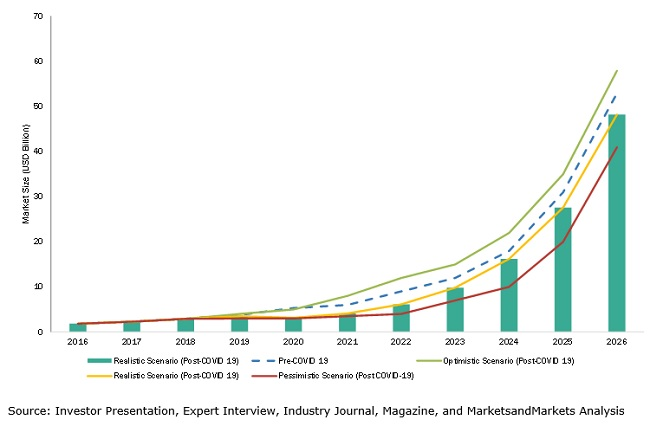
\includegraphics[width=1.0\linewidth]{img/digital-twin-market12.jpg}
    \caption[Übersicht Marktgröße \ac{DT}]{Marktentwicklung und Marktvorhersage für den Markt digitlaer Zwillinge \\Quelle: \citeauthor{markets2020} \citeurl{markets2020}} 
\end{figure}


Die Industrie ist allerdings nicht der einzige Ort, an dem \ac{DT}s vorteilhaft eingesetzt werden und wurden. Der Bereich der \ac{PHM} profitiert auch von der Nutzung digitaler Zwillinge. \citeauthor{tuegel2011reengineering} beschrieb bereits im Jahr \citeyear{tuegel2011reengineering} den Einsatz von \ac{DT}s zur Vorhersage des Lebenszyklus von Luftfahrzeugen. Dabei konnte durch die Abbildung in einer virtuellen Umgebung komplexe zusammenhängende Physiksimulationen durchgeführt werden. Damit konnten Vereinfachungen in verscheidenen Bereichen der Wartung eines Luftfahrzeugs erreicht werden.\autocites{tao2018digital}{tuegel2011reengineering} \\
Des weiteren lassen sich Forschungen für Anwendung im medizinischen Bereich finden. \autocites{barricelli2019survey}{tao2018digital}

\pagebreak

Große weltweit agierende Unternehmen, erkennen und fördern den gewonnenen Nutzen durch \ac{DT}s. Dazu zählen Unternehmen wie:
\begin{itemize}
    \item \textbf{Siemens:}\\ Siemens nutzt digitale Zwillinge im Bereich von Strom- und Abwasseranlagen in Finnland. Dort dienen die \ac{DT}s dazu, interne Abläufe zu optimieren und zu automatisieren.\autocite{tao2018digital}
    \item \textbf{Airbus:}\\ Airbus erreicht mithilfe von \ac{DT}s einen sehr hohen Automatisierungsgrad innerhalb der eigenen Fabriken. Konkret werden dort digitale Zwillinge eingesetzt, um Produktionslinien abzubilden, um so den Fertigungsgrad zu überwachen und Prozesse zu optimieren \autocite{tao2018digital}
    \item \textbf{Bosch:}\\ Bosch ist vor allem im Bereich der Softwareentwicklung für digitale Zwillinge tätig und bietet eine eigene Cloudlösung zur Verwaltung von \ac{DT}s an. Außerdem stellen sie viele Entwickler für verscheidene Eclipse Projekte bereit. \autocite{tao2018digital}
    \item \textbf{SAP SE:}\\ Die SAP SE kann durch digitale Zwillinge das \ac{PHM} von Unterwasseranlagen überwachen und Fernwartungen/-diagnosen durchführen. Somit entsteht eine immense Kostenersparnis, da Wartungseinsätze unter Wasser teuer sind. \autocite{tao2018digital}
\end{itemize}


